\documentclass[aspectratio=169]{beamer}
% Shared preamble for ml/ slide decks.
% Each lecture .tex starts with:
%   \documentclass[aspectratio=169]{beamer}
%   % Shared preamble for ml/ slide decks.
% Each lecture .tex starts with:
%   \documentclass[aspectratio=169]{beamer}
%   % Shared preamble for ml/ slide decks.
% Each lecture .tex starts with:
%   \documentclass[aspectratio=169]{beamer}
%   \input{../preamble}
% Compile from inside the chapter folder so \input{../preamble} resolves.

\usetheme{default}
\usecolortheme{dove}

\setbeamertemplate{navigation symbols}{}
\setbeamertemplate{footline}{%
  \hfill{\large\insertframenumber\,/\,\inserttotalframenumber}\hspace{0.8em}\vspace{0.5em}%
}

% Project palette (existing, kept for backwards compatibility with deferred/*)
\definecolor{popblue}{RGB}{52, 101, 164}
\definecolor{sampred}{RGB}{204, 0, 0}
\definecolor{paramgreen}{RGB}{0, 140, 70}
\definecolor{warnred}{RGB}{180, 40, 40}
\definecolor{orange1}{RGB}{220, 120, 0}
\definecolor{violet1}{RGB}{120, 50, 160}
\definecolor{lightbg}{RGB}{245, 245, 250}

% Armenian flag palette (use these for any 3-color highlight; per CLAUDE.md).
% "Nice versions": slightly de-saturated from the official spec for slide use,
% so they don't burn out under projector colors. Originals kept as *_pure.
\definecolor{armred}{RGB}{200, 30, 40}      % nice red (official #D90012 muted)
\definecolor{armblue}{RGB}{30, 70, 160}     % nice blue (official #0033A0 muted)
\definecolor{armorange}{RGB}{230, 160, 30}  % nice orange (official #F2A800 muted)
\definecolor{armred_pure}{HTML}{D90012}     % official Armenian flag red
\definecolor{armblue_pure}{HTML}{0033A0}    % official Armenian flag blue
\definecolor{armorange_pure}{HTML}{F2A800}  % official Armenian flag orange

\setbeamercolor{frametitle}{fg=popblue}
\setbeamercolor{title}{fg=popblue}

\usepackage{pgfplots}
\usepackage{tikz}
\usetikzlibrary{shapes, arrows.meta, positioning, calc, decorations.pathreplacing, patterns, matrix}
\pgfplotsset{compat=1.18}
\usepackage{amsmath, amssymb, amsfonts}
\usepackage{bm}
\usepackage{dsfont}
\usepackage{array}
\usepackage{pifont}
\usepackage{colortbl}
\usepackage{fontenc}

% Callout boxes. Purely additive - existing decks are unaffected.
% Usage: \begin{tcolorbox}[colback=armblue!8, colframe=armblue, boxrule=0.6pt, arc=2pt,
%                          title=\textbf{Key idea}] ... \end{tcolorbox}
% Palette convention (ml/SLIDE_STYLE.md): armblue=key idea, armred=trap/warning,
% paramgreen=takeaway or "Next", armorange=watch-out.
\usepackage[most]{tcolorbox}

% Cleaner table rules (\toprule, \midrule, \bottomrule). Also purely additive.
\usepackage{booktabs}

% \cancel{...} for struck-through terms in derivations (added 2026-08-11 for the
% importance-sampling frame in ch11_rl, where the dynamics cancel). Purely additive.
\usepackage{cancel}

% Minimal ML notation macros (subset of slds-lmu latex-math/basic-ml.tex).
% Kept here so we don't have to inline-expand every \thetav, \xv, etc.
% when porting upstream slides.
\newcommand{\R}{\mathds{R}}
\newcommand{\N}{\mathds{N}}
\newcommand{\E}{\mathds{E}}
\newcommand{\Xspace}{\mathcal{X}}
\newcommand{\Yspace}{\mathcal{Y}}
\newcommand{\Hspace}{\mathcal{H}}
\newcommand{\D}{\mathcal{D}}
\newcommand{\Dtrain}{\mathcal{D}_{\text{train}}}
\newcommand{\Dtest}{\mathcal{D}_{\text{test}}}
\newcommand{\xv}{\mathbf{x}}
\newcommand{\yv}{\mathbf{y}}
\newcommand{\Xmat}{\mathbf{X}}
\newcommand{\id}{\mathbf{I}}
\newcommand{\thetav}{\bm{\theta}}
\newcommand{\thetah}{\hat{\bm{\theta}}}
\newcommand{\lamv}{\bm{\lambda}}
\newcommand{\fx}{f(\xv)}
\newcommand{\fxt}{f(\xv \,|\, \bm{\theta})}
\newcommand{\fxi}{f\!\left(\xv^{(i)}\right)}
\newcommand{\fh}{\hat{f}}
\newcommand{\fxh}{\hat{f}(\xv)}
\newcommand{\yh}{\hat{y}}
\newcommand{\yih}{\hat{y}^{(i)}}
% \xi clashes with the Greek letter \xi; write \xv^{(i)} inline instead.
\newcommand{\yi}[1][i]{y^{(#1)}}
\newcommand{\xyi}[1][i]{\left(\xv^{(#1)},\, y^{(#1)}\right)}
\newcommand{\thx}{\bm{\theta}^\top \xv}
\newcommand{\sumin}{\sum_{i=1}^{n}}
\newcommand{\sumjp}{\sum_{j=1}^{p}}
\newcommand{\Lxy}{L\!\left(y, \fx\right)}
\newcommand{\Lxyi}{L\!\left(\yi, \fxi\right)}
\newcommand{\risk}{\mathcal{R}}
\newcommand{\riske}{\mathcal{R}_{\text{emp}}}
\newcommand{\risket}{\mathcal{R}_{\text{emp}}(\bm{\theta})}
\newcommand{\riskt}{\mathcal{R}(\bm{\theta})}
\newcommand{\riskr}{\mathcal{R}_{\text{reg}}}
\newcommand{\argmin}{\mathop{\mathrm{arg\,min}}}
\newcommand{\argmax}{\mathop{\mathrm{arg\,max}}}
\newcommand{\eps}{\varepsilon}

% Compile from inside the chapter folder so % Shared preamble for ml/ slide decks.
% Each lecture .tex starts with:
%   \documentclass[aspectratio=169]{beamer}
%   \input{../preamble}
% Compile from inside the chapter folder so \input{../preamble} resolves.

\usetheme{default}
\usecolortheme{dove}

\setbeamertemplate{navigation symbols}{}
\setbeamertemplate{footline}{%
  \hfill{\large\insertframenumber\,/\,\inserttotalframenumber}\hspace{0.8em}\vspace{0.5em}%
}

% Project palette (existing, kept for backwards compatibility with deferred/*)
\definecolor{popblue}{RGB}{52, 101, 164}
\definecolor{sampred}{RGB}{204, 0, 0}
\definecolor{paramgreen}{RGB}{0, 140, 70}
\definecolor{warnred}{RGB}{180, 40, 40}
\definecolor{orange1}{RGB}{220, 120, 0}
\definecolor{violet1}{RGB}{120, 50, 160}
\definecolor{lightbg}{RGB}{245, 245, 250}

% Armenian flag palette (use these for any 3-color highlight; per CLAUDE.md).
% "Nice versions": slightly de-saturated from the official spec for slide use,
% so they don't burn out under projector colors. Originals kept as *_pure.
\definecolor{armred}{RGB}{200, 30, 40}      % nice red (official #D90012 muted)
\definecolor{armblue}{RGB}{30, 70, 160}     % nice blue (official #0033A0 muted)
\definecolor{armorange}{RGB}{230, 160, 30}  % nice orange (official #F2A800 muted)
\definecolor{armred_pure}{HTML}{D90012}     % official Armenian flag red
\definecolor{armblue_pure}{HTML}{0033A0}    % official Armenian flag blue
\definecolor{armorange_pure}{HTML}{F2A800}  % official Armenian flag orange

\setbeamercolor{frametitle}{fg=popblue}
\setbeamercolor{title}{fg=popblue}

\usepackage{pgfplots}
\usepackage{tikz}
\usetikzlibrary{shapes, arrows.meta, positioning, calc, decorations.pathreplacing, patterns, matrix}
\pgfplotsset{compat=1.18}
\usepackage{amsmath, amssymb, amsfonts}
\usepackage{bm}
\usepackage{dsfont}
\usepackage{array}
\usepackage{pifont}
\usepackage{colortbl}
\usepackage{fontenc}

% Callout boxes. Purely additive - existing decks are unaffected.
% Usage: \begin{tcolorbox}[colback=armblue!8, colframe=armblue, boxrule=0.6pt, arc=2pt,
%                          title=\textbf{Key idea}] ... \end{tcolorbox}
% Palette convention (ml/SLIDE_STYLE.md): armblue=key idea, armred=trap/warning,
% paramgreen=takeaway or "Next", armorange=watch-out.
\usepackage[most]{tcolorbox}

% Cleaner table rules (\toprule, \midrule, \bottomrule). Also purely additive.
\usepackage{booktabs}

% \cancel{...} for struck-through terms in derivations (added 2026-08-11 for the
% importance-sampling frame in ch11_rl, where the dynamics cancel). Purely additive.
\usepackage{cancel}

% Minimal ML notation macros (subset of slds-lmu latex-math/basic-ml.tex).
% Kept here so we don't have to inline-expand every \thetav, \xv, etc.
% when porting upstream slides.
\newcommand{\R}{\mathds{R}}
\newcommand{\N}{\mathds{N}}
\newcommand{\E}{\mathds{E}}
\newcommand{\Xspace}{\mathcal{X}}
\newcommand{\Yspace}{\mathcal{Y}}
\newcommand{\Hspace}{\mathcal{H}}
\newcommand{\D}{\mathcal{D}}
\newcommand{\Dtrain}{\mathcal{D}_{\text{train}}}
\newcommand{\Dtest}{\mathcal{D}_{\text{test}}}
\newcommand{\xv}{\mathbf{x}}
\newcommand{\yv}{\mathbf{y}}
\newcommand{\Xmat}{\mathbf{X}}
\newcommand{\id}{\mathbf{I}}
\newcommand{\thetav}{\bm{\theta}}
\newcommand{\thetah}{\hat{\bm{\theta}}}
\newcommand{\lamv}{\bm{\lambda}}
\newcommand{\fx}{f(\xv)}
\newcommand{\fxt}{f(\xv \,|\, \bm{\theta})}
\newcommand{\fxi}{f\!\left(\xv^{(i)}\right)}
\newcommand{\fh}{\hat{f}}
\newcommand{\fxh}{\hat{f}(\xv)}
\newcommand{\yh}{\hat{y}}
\newcommand{\yih}{\hat{y}^{(i)}}
% \xi clashes with the Greek letter \xi; write \xv^{(i)} inline instead.
\newcommand{\yi}[1][i]{y^{(#1)}}
\newcommand{\xyi}[1][i]{\left(\xv^{(#1)},\, y^{(#1)}\right)}
\newcommand{\thx}{\bm{\theta}^\top \xv}
\newcommand{\sumin}{\sum_{i=1}^{n}}
\newcommand{\sumjp}{\sum_{j=1}^{p}}
\newcommand{\Lxy}{L\!\left(y, \fx\right)}
\newcommand{\Lxyi}{L\!\left(\yi, \fxi\right)}
\newcommand{\risk}{\mathcal{R}}
\newcommand{\riske}{\mathcal{R}_{\text{emp}}}
\newcommand{\risket}{\mathcal{R}_{\text{emp}}(\bm{\theta})}
\newcommand{\riskt}{\mathcal{R}(\bm{\theta})}
\newcommand{\riskr}{\mathcal{R}_{\text{reg}}}
\newcommand{\argmin}{\mathop{\mathrm{arg\,min}}}
\newcommand{\argmax}{\mathop{\mathrm{arg\,max}}}
\newcommand{\eps}{\varepsilon}
 resolves.

\usetheme{default}
\usecolortheme{dove}

\setbeamertemplate{navigation symbols}{}
\setbeamertemplate{footline}{%
  \hfill{\large\insertframenumber\,/\,\inserttotalframenumber}\hspace{0.8em}\vspace{0.5em}%
}

% Project palette (existing, kept for backwards compatibility with deferred/*)
\definecolor{popblue}{RGB}{52, 101, 164}
\definecolor{sampred}{RGB}{204, 0, 0}
\definecolor{paramgreen}{RGB}{0, 140, 70}
\definecolor{warnred}{RGB}{180, 40, 40}
\definecolor{orange1}{RGB}{220, 120, 0}
\definecolor{violet1}{RGB}{120, 50, 160}
\definecolor{lightbg}{RGB}{245, 245, 250}

% Armenian flag palette (use these for any 3-color highlight; per CLAUDE.md).
% "Nice versions": slightly de-saturated from the official spec for slide use,
% so they don't burn out under projector colors. Originals kept as *_pure.
\definecolor{armred}{RGB}{200, 30, 40}      % nice red (official #D90012 muted)
\definecolor{armblue}{RGB}{30, 70, 160}     % nice blue (official #0033A0 muted)
\definecolor{armorange}{RGB}{230, 160, 30}  % nice orange (official #F2A800 muted)
\definecolor{armred_pure}{HTML}{D90012}     % official Armenian flag red
\definecolor{armblue_pure}{HTML}{0033A0}    % official Armenian flag blue
\definecolor{armorange_pure}{HTML}{F2A800}  % official Armenian flag orange

\setbeamercolor{frametitle}{fg=popblue}
\setbeamercolor{title}{fg=popblue}

\usepackage{pgfplots}
\usepackage{tikz}
\usetikzlibrary{shapes, arrows.meta, positioning, calc, decorations.pathreplacing, patterns, matrix}
\pgfplotsset{compat=1.18}
\usepackage{amsmath, amssymb, amsfonts}
\usepackage{bm}
\usepackage{dsfont}
\usepackage{array}
\usepackage{pifont}
\usepackage{colortbl}
\usepackage{fontenc}

% Callout boxes. Purely additive - existing decks are unaffected.
% Usage: \begin{tcolorbox}[colback=armblue!8, colframe=armblue, boxrule=0.6pt, arc=2pt,
%                          title=\textbf{Key idea}] ... \end{tcolorbox}
% Palette convention (ml/SLIDE_STYLE.md): armblue=key idea, armred=trap/warning,
% paramgreen=takeaway or "Next", armorange=watch-out.
\usepackage[most]{tcolorbox}

% Cleaner table rules (\toprule, \midrule, \bottomrule). Also purely additive.
\usepackage{booktabs}

% \cancel{...} for struck-through terms in derivations (added 2026-08-11 for the
% importance-sampling frame in ch11_rl, where the dynamics cancel). Purely additive.
\usepackage{cancel}

% Minimal ML notation macros (subset of slds-lmu latex-math/basic-ml.tex).
% Kept here so we don't have to inline-expand every \thetav, \xv, etc.
% when porting upstream slides.
\newcommand{\R}{\mathds{R}}
\newcommand{\N}{\mathds{N}}
\newcommand{\E}{\mathds{E}}
\newcommand{\Xspace}{\mathcal{X}}
\newcommand{\Yspace}{\mathcal{Y}}
\newcommand{\Hspace}{\mathcal{H}}
\newcommand{\D}{\mathcal{D}}
\newcommand{\Dtrain}{\mathcal{D}_{\text{train}}}
\newcommand{\Dtest}{\mathcal{D}_{\text{test}}}
\newcommand{\xv}{\mathbf{x}}
\newcommand{\yv}{\mathbf{y}}
\newcommand{\Xmat}{\mathbf{X}}
\newcommand{\id}{\mathbf{I}}
\newcommand{\thetav}{\bm{\theta}}
\newcommand{\thetah}{\hat{\bm{\theta}}}
\newcommand{\lamv}{\bm{\lambda}}
\newcommand{\fx}{f(\xv)}
\newcommand{\fxt}{f(\xv \,|\, \bm{\theta})}
\newcommand{\fxi}{f\!\left(\xv^{(i)}\right)}
\newcommand{\fh}{\hat{f}}
\newcommand{\fxh}{\hat{f}(\xv)}
\newcommand{\yh}{\hat{y}}
\newcommand{\yih}{\hat{y}^{(i)}}
% \xi clashes with the Greek letter \xi; write \xv^{(i)} inline instead.
\newcommand{\yi}[1][i]{y^{(#1)}}
\newcommand{\xyi}[1][i]{\left(\xv^{(#1)},\, y^{(#1)}\right)}
\newcommand{\thx}{\bm{\theta}^\top \xv}
\newcommand{\sumin}{\sum_{i=1}^{n}}
\newcommand{\sumjp}{\sum_{j=1}^{p}}
\newcommand{\Lxy}{L\!\left(y, \fx\right)}
\newcommand{\Lxyi}{L\!\left(\yi, \fxi\right)}
\newcommand{\risk}{\mathcal{R}}
\newcommand{\riske}{\mathcal{R}_{\text{emp}}}
\newcommand{\risket}{\mathcal{R}_{\text{emp}}(\bm{\theta})}
\newcommand{\riskt}{\mathcal{R}(\bm{\theta})}
\newcommand{\riskr}{\mathcal{R}_{\text{reg}}}
\newcommand{\argmin}{\mathop{\mathrm{arg\,min}}}
\newcommand{\argmax}{\mathop{\mathrm{arg\,max}}}
\newcommand{\eps}{\varepsilon}

% Compile from inside the chapter folder so % Shared preamble for ml/ slide decks.
% Each lecture .tex starts with:
%   \documentclass[aspectratio=169]{beamer}
%   % Shared preamble for ml/ slide decks.
% Each lecture .tex starts with:
%   \documentclass[aspectratio=169]{beamer}
%   \input{../preamble}
% Compile from inside the chapter folder so \input{../preamble} resolves.

\usetheme{default}
\usecolortheme{dove}

\setbeamertemplate{navigation symbols}{}
\setbeamertemplate{footline}{%
  \hfill{\large\insertframenumber\,/\,\inserttotalframenumber}\hspace{0.8em}\vspace{0.5em}%
}

% Project palette (existing, kept for backwards compatibility with deferred/*)
\definecolor{popblue}{RGB}{52, 101, 164}
\definecolor{sampred}{RGB}{204, 0, 0}
\definecolor{paramgreen}{RGB}{0, 140, 70}
\definecolor{warnred}{RGB}{180, 40, 40}
\definecolor{orange1}{RGB}{220, 120, 0}
\definecolor{violet1}{RGB}{120, 50, 160}
\definecolor{lightbg}{RGB}{245, 245, 250}

% Armenian flag palette (use these for any 3-color highlight; per CLAUDE.md).
% "Nice versions": slightly de-saturated from the official spec for slide use,
% so they don't burn out under projector colors. Originals kept as *_pure.
\definecolor{armred}{RGB}{200, 30, 40}      % nice red (official #D90012 muted)
\definecolor{armblue}{RGB}{30, 70, 160}     % nice blue (official #0033A0 muted)
\definecolor{armorange}{RGB}{230, 160, 30}  % nice orange (official #F2A800 muted)
\definecolor{armred_pure}{HTML}{D90012}     % official Armenian flag red
\definecolor{armblue_pure}{HTML}{0033A0}    % official Armenian flag blue
\definecolor{armorange_pure}{HTML}{F2A800}  % official Armenian flag orange

\setbeamercolor{frametitle}{fg=popblue}
\setbeamercolor{title}{fg=popblue}

\usepackage{pgfplots}
\usepackage{tikz}
\usetikzlibrary{shapes, arrows.meta, positioning, calc, decorations.pathreplacing, patterns, matrix}
\pgfplotsset{compat=1.18}
\usepackage{amsmath, amssymb, amsfonts}
\usepackage{bm}
\usepackage{dsfont}
\usepackage{array}
\usepackage{pifont}
\usepackage{colortbl}
\usepackage{fontenc}

% Callout boxes. Purely additive - existing decks are unaffected.
% Usage: \begin{tcolorbox}[colback=armblue!8, colframe=armblue, boxrule=0.6pt, arc=2pt,
%                          title=\textbf{Key idea}] ... \end{tcolorbox}
% Palette convention (ml/SLIDE_STYLE.md): armblue=key idea, armred=trap/warning,
% paramgreen=takeaway or "Next", armorange=watch-out.
\usepackage[most]{tcolorbox}

% Cleaner table rules (\toprule, \midrule, \bottomrule). Also purely additive.
\usepackage{booktabs}

% \cancel{...} for struck-through terms in derivations (added 2026-08-11 for the
% importance-sampling frame in ch11_rl, where the dynamics cancel). Purely additive.
\usepackage{cancel}

% Minimal ML notation macros (subset of slds-lmu latex-math/basic-ml.tex).
% Kept here so we don't have to inline-expand every \thetav, \xv, etc.
% when porting upstream slides.
\newcommand{\R}{\mathds{R}}
\newcommand{\N}{\mathds{N}}
\newcommand{\E}{\mathds{E}}
\newcommand{\Xspace}{\mathcal{X}}
\newcommand{\Yspace}{\mathcal{Y}}
\newcommand{\Hspace}{\mathcal{H}}
\newcommand{\D}{\mathcal{D}}
\newcommand{\Dtrain}{\mathcal{D}_{\text{train}}}
\newcommand{\Dtest}{\mathcal{D}_{\text{test}}}
\newcommand{\xv}{\mathbf{x}}
\newcommand{\yv}{\mathbf{y}}
\newcommand{\Xmat}{\mathbf{X}}
\newcommand{\id}{\mathbf{I}}
\newcommand{\thetav}{\bm{\theta}}
\newcommand{\thetah}{\hat{\bm{\theta}}}
\newcommand{\lamv}{\bm{\lambda}}
\newcommand{\fx}{f(\xv)}
\newcommand{\fxt}{f(\xv \,|\, \bm{\theta})}
\newcommand{\fxi}{f\!\left(\xv^{(i)}\right)}
\newcommand{\fh}{\hat{f}}
\newcommand{\fxh}{\hat{f}(\xv)}
\newcommand{\yh}{\hat{y}}
\newcommand{\yih}{\hat{y}^{(i)}}
% \xi clashes with the Greek letter \xi; write \xv^{(i)} inline instead.
\newcommand{\yi}[1][i]{y^{(#1)}}
\newcommand{\xyi}[1][i]{\left(\xv^{(#1)},\, y^{(#1)}\right)}
\newcommand{\thx}{\bm{\theta}^\top \xv}
\newcommand{\sumin}{\sum_{i=1}^{n}}
\newcommand{\sumjp}{\sum_{j=1}^{p}}
\newcommand{\Lxy}{L\!\left(y, \fx\right)}
\newcommand{\Lxyi}{L\!\left(\yi, \fxi\right)}
\newcommand{\risk}{\mathcal{R}}
\newcommand{\riske}{\mathcal{R}_{\text{emp}}}
\newcommand{\risket}{\mathcal{R}_{\text{emp}}(\bm{\theta})}
\newcommand{\riskt}{\mathcal{R}(\bm{\theta})}
\newcommand{\riskr}{\mathcal{R}_{\text{reg}}}
\newcommand{\argmin}{\mathop{\mathrm{arg\,min}}}
\newcommand{\argmax}{\mathop{\mathrm{arg\,max}}}
\newcommand{\eps}{\varepsilon}

% Compile from inside the chapter folder so % Shared preamble for ml/ slide decks.
% Each lecture .tex starts with:
%   \documentclass[aspectratio=169]{beamer}
%   \input{../preamble}
% Compile from inside the chapter folder so \input{../preamble} resolves.

\usetheme{default}
\usecolortheme{dove}

\setbeamertemplate{navigation symbols}{}
\setbeamertemplate{footline}{%
  \hfill{\large\insertframenumber\,/\,\inserttotalframenumber}\hspace{0.8em}\vspace{0.5em}%
}

% Project palette (existing, kept for backwards compatibility with deferred/*)
\definecolor{popblue}{RGB}{52, 101, 164}
\definecolor{sampred}{RGB}{204, 0, 0}
\definecolor{paramgreen}{RGB}{0, 140, 70}
\definecolor{warnred}{RGB}{180, 40, 40}
\definecolor{orange1}{RGB}{220, 120, 0}
\definecolor{violet1}{RGB}{120, 50, 160}
\definecolor{lightbg}{RGB}{245, 245, 250}

% Armenian flag palette (use these for any 3-color highlight; per CLAUDE.md).
% "Nice versions": slightly de-saturated from the official spec for slide use,
% so they don't burn out under projector colors. Originals kept as *_pure.
\definecolor{armred}{RGB}{200, 30, 40}      % nice red (official #D90012 muted)
\definecolor{armblue}{RGB}{30, 70, 160}     % nice blue (official #0033A0 muted)
\definecolor{armorange}{RGB}{230, 160, 30}  % nice orange (official #F2A800 muted)
\definecolor{armred_pure}{HTML}{D90012}     % official Armenian flag red
\definecolor{armblue_pure}{HTML}{0033A0}    % official Armenian flag blue
\definecolor{armorange_pure}{HTML}{F2A800}  % official Armenian flag orange

\setbeamercolor{frametitle}{fg=popblue}
\setbeamercolor{title}{fg=popblue}

\usepackage{pgfplots}
\usepackage{tikz}
\usetikzlibrary{shapes, arrows.meta, positioning, calc, decorations.pathreplacing, patterns, matrix}
\pgfplotsset{compat=1.18}
\usepackage{amsmath, amssymb, amsfonts}
\usepackage{bm}
\usepackage{dsfont}
\usepackage{array}
\usepackage{pifont}
\usepackage{colortbl}
\usepackage{fontenc}

% Callout boxes. Purely additive - existing decks are unaffected.
% Usage: \begin{tcolorbox}[colback=armblue!8, colframe=armblue, boxrule=0.6pt, arc=2pt,
%                          title=\textbf{Key idea}] ... \end{tcolorbox}
% Palette convention (ml/SLIDE_STYLE.md): armblue=key idea, armred=trap/warning,
% paramgreen=takeaway or "Next", armorange=watch-out.
\usepackage[most]{tcolorbox}

% Cleaner table rules (\toprule, \midrule, \bottomrule). Also purely additive.
\usepackage{booktabs}

% \cancel{...} for struck-through terms in derivations (added 2026-08-11 for the
% importance-sampling frame in ch11_rl, where the dynamics cancel). Purely additive.
\usepackage{cancel}

% Minimal ML notation macros (subset of slds-lmu latex-math/basic-ml.tex).
% Kept here so we don't have to inline-expand every \thetav, \xv, etc.
% when porting upstream slides.
\newcommand{\R}{\mathds{R}}
\newcommand{\N}{\mathds{N}}
\newcommand{\E}{\mathds{E}}
\newcommand{\Xspace}{\mathcal{X}}
\newcommand{\Yspace}{\mathcal{Y}}
\newcommand{\Hspace}{\mathcal{H}}
\newcommand{\D}{\mathcal{D}}
\newcommand{\Dtrain}{\mathcal{D}_{\text{train}}}
\newcommand{\Dtest}{\mathcal{D}_{\text{test}}}
\newcommand{\xv}{\mathbf{x}}
\newcommand{\yv}{\mathbf{y}}
\newcommand{\Xmat}{\mathbf{X}}
\newcommand{\id}{\mathbf{I}}
\newcommand{\thetav}{\bm{\theta}}
\newcommand{\thetah}{\hat{\bm{\theta}}}
\newcommand{\lamv}{\bm{\lambda}}
\newcommand{\fx}{f(\xv)}
\newcommand{\fxt}{f(\xv \,|\, \bm{\theta})}
\newcommand{\fxi}{f\!\left(\xv^{(i)}\right)}
\newcommand{\fh}{\hat{f}}
\newcommand{\fxh}{\hat{f}(\xv)}
\newcommand{\yh}{\hat{y}}
\newcommand{\yih}{\hat{y}^{(i)}}
% \xi clashes with the Greek letter \xi; write \xv^{(i)} inline instead.
\newcommand{\yi}[1][i]{y^{(#1)}}
\newcommand{\xyi}[1][i]{\left(\xv^{(#1)},\, y^{(#1)}\right)}
\newcommand{\thx}{\bm{\theta}^\top \xv}
\newcommand{\sumin}{\sum_{i=1}^{n}}
\newcommand{\sumjp}{\sum_{j=1}^{p}}
\newcommand{\Lxy}{L\!\left(y, \fx\right)}
\newcommand{\Lxyi}{L\!\left(\yi, \fxi\right)}
\newcommand{\risk}{\mathcal{R}}
\newcommand{\riske}{\mathcal{R}_{\text{emp}}}
\newcommand{\risket}{\mathcal{R}_{\text{emp}}(\bm{\theta})}
\newcommand{\riskt}{\mathcal{R}(\bm{\theta})}
\newcommand{\riskr}{\mathcal{R}_{\text{reg}}}
\newcommand{\argmin}{\mathop{\mathrm{arg\,min}}}
\newcommand{\argmax}{\mathop{\mathrm{arg\,max}}}
\newcommand{\eps}{\varepsilon}
 resolves.

\usetheme{default}
\usecolortheme{dove}

\setbeamertemplate{navigation symbols}{}
\setbeamertemplate{footline}{%
  \hfill{\large\insertframenumber\,/\,\inserttotalframenumber}\hspace{0.8em}\vspace{0.5em}%
}

% Project palette (existing, kept for backwards compatibility with deferred/*)
\definecolor{popblue}{RGB}{52, 101, 164}
\definecolor{sampred}{RGB}{204, 0, 0}
\definecolor{paramgreen}{RGB}{0, 140, 70}
\definecolor{warnred}{RGB}{180, 40, 40}
\definecolor{orange1}{RGB}{220, 120, 0}
\definecolor{violet1}{RGB}{120, 50, 160}
\definecolor{lightbg}{RGB}{245, 245, 250}

% Armenian flag palette (use these for any 3-color highlight; per CLAUDE.md).
% "Nice versions": slightly de-saturated from the official spec for slide use,
% so they don't burn out under projector colors. Originals kept as *_pure.
\definecolor{armred}{RGB}{200, 30, 40}      % nice red (official #D90012 muted)
\definecolor{armblue}{RGB}{30, 70, 160}     % nice blue (official #0033A0 muted)
\definecolor{armorange}{RGB}{230, 160, 30}  % nice orange (official #F2A800 muted)
\definecolor{armred_pure}{HTML}{D90012}     % official Armenian flag red
\definecolor{armblue_pure}{HTML}{0033A0}    % official Armenian flag blue
\definecolor{armorange_pure}{HTML}{F2A800}  % official Armenian flag orange

\setbeamercolor{frametitle}{fg=popblue}
\setbeamercolor{title}{fg=popblue}

\usepackage{pgfplots}
\usepackage{tikz}
\usetikzlibrary{shapes, arrows.meta, positioning, calc, decorations.pathreplacing, patterns, matrix}
\pgfplotsset{compat=1.18}
\usepackage{amsmath, amssymb, amsfonts}
\usepackage{bm}
\usepackage{dsfont}
\usepackage{array}
\usepackage{pifont}
\usepackage{colortbl}
\usepackage{fontenc}

% Callout boxes. Purely additive - existing decks are unaffected.
% Usage: \begin{tcolorbox}[colback=armblue!8, colframe=armblue, boxrule=0.6pt, arc=2pt,
%                          title=\textbf{Key idea}] ... \end{tcolorbox}
% Palette convention (ml/SLIDE_STYLE.md): armblue=key idea, armred=trap/warning,
% paramgreen=takeaway or "Next", armorange=watch-out.
\usepackage[most]{tcolorbox}

% Cleaner table rules (\toprule, \midrule, \bottomrule). Also purely additive.
\usepackage{booktabs}

% \cancel{...} for struck-through terms in derivations (added 2026-08-11 for the
% importance-sampling frame in ch11_rl, where the dynamics cancel). Purely additive.
\usepackage{cancel}

% Minimal ML notation macros (subset of slds-lmu latex-math/basic-ml.tex).
% Kept here so we don't have to inline-expand every \thetav, \xv, etc.
% when porting upstream slides.
\newcommand{\R}{\mathds{R}}
\newcommand{\N}{\mathds{N}}
\newcommand{\E}{\mathds{E}}
\newcommand{\Xspace}{\mathcal{X}}
\newcommand{\Yspace}{\mathcal{Y}}
\newcommand{\Hspace}{\mathcal{H}}
\newcommand{\D}{\mathcal{D}}
\newcommand{\Dtrain}{\mathcal{D}_{\text{train}}}
\newcommand{\Dtest}{\mathcal{D}_{\text{test}}}
\newcommand{\xv}{\mathbf{x}}
\newcommand{\yv}{\mathbf{y}}
\newcommand{\Xmat}{\mathbf{X}}
\newcommand{\id}{\mathbf{I}}
\newcommand{\thetav}{\bm{\theta}}
\newcommand{\thetah}{\hat{\bm{\theta}}}
\newcommand{\lamv}{\bm{\lambda}}
\newcommand{\fx}{f(\xv)}
\newcommand{\fxt}{f(\xv \,|\, \bm{\theta})}
\newcommand{\fxi}{f\!\left(\xv^{(i)}\right)}
\newcommand{\fh}{\hat{f}}
\newcommand{\fxh}{\hat{f}(\xv)}
\newcommand{\yh}{\hat{y}}
\newcommand{\yih}{\hat{y}^{(i)}}
% \xi clashes with the Greek letter \xi; write \xv^{(i)} inline instead.
\newcommand{\yi}[1][i]{y^{(#1)}}
\newcommand{\xyi}[1][i]{\left(\xv^{(#1)},\, y^{(#1)}\right)}
\newcommand{\thx}{\bm{\theta}^\top \xv}
\newcommand{\sumin}{\sum_{i=1}^{n}}
\newcommand{\sumjp}{\sum_{j=1}^{p}}
\newcommand{\Lxy}{L\!\left(y, \fx\right)}
\newcommand{\Lxyi}{L\!\left(\yi, \fxi\right)}
\newcommand{\risk}{\mathcal{R}}
\newcommand{\riske}{\mathcal{R}_{\text{emp}}}
\newcommand{\risket}{\mathcal{R}_{\text{emp}}(\bm{\theta})}
\newcommand{\riskt}{\mathcal{R}(\bm{\theta})}
\newcommand{\riskr}{\mathcal{R}_{\text{reg}}}
\newcommand{\argmin}{\mathop{\mathrm{arg\,min}}}
\newcommand{\argmax}{\mathop{\mathrm{arg\,max}}}
\newcommand{\eps}{\varepsilon}
 resolves.

\usetheme{default}
\usecolortheme{dove}

\setbeamertemplate{navigation symbols}{}
\setbeamertemplate{footline}{%
  \hfill{\large\insertframenumber\,/\,\inserttotalframenumber}\hspace{0.8em}\vspace{0.5em}%
}

% Project palette (existing, kept for backwards compatibility with deferred/*)
\definecolor{popblue}{RGB}{52, 101, 164}
\definecolor{sampred}{RGB}{204, 0, 0}
\definecolor{paramgreen}{RGB}{0, 140, 70}
\definecolor{warnred}{RGB}{180, 40, 40}
\definecolor{orange1}{RGB}{220, 120, 0}
\definecolor{violet1}{RGB}{120, 50, 160}
\definecolor{lightbg}{RGB}{245, 245, 250}

% Armenian flag palette (use these for any 3-color highlight; per CLAUDE.md).
% "Nice versions": slightly de-saturated from the official spec for slide use,
% so they don't burn out under projector colors. Originals kept as *_pure.
\definecolor{armred}{RGB}{200, 30, 40}      % nice red (official #D90012 muted)
\definecolor{armblue}{RGB}{30, 70, 160}     % nice blue (official #0033A0 muted)
\definecolor{armorange}{RGB}{230, 160, 30}  % nice orange (official #F2A800 muted)
\definecolor{armred_pure}{HTML}{D90012}     % official Armenian flag red
\definecolor{armblue_pure}{HTML}{0033A0}    % official Armenian flag blue
\definecolor{armorange_pure}{HTML}{F2A800}  % official Armenian flag orange

\setbeamercolor{frametitle}{fg=popblue}
\setbeamercolor{title}{fg=popblue}

\usepackage{pgfplots}
\usepackage{tikz}
\usetikzlibrary{shapes, arrows.meta, positioning, calc, decorations.pathreplacing, patterns, matrix}
\pgfplotsset{compat=1.18}
\usepackage{amsmath, amssymb, amsfonts}
\usepackage{bm}
\usepackage{dsfont}
\usepackage{array}
\usepackage{pifont}
\usepackage{colortbl}
\usepackage{fontenc}

% Callout boxes. Purely additive - existing decks are unaffected.
% Usage: \begin{tcolorbox}[colback=armblue!8, colframe=armblue, boxrule=0.6pt, arc=2pt,
%                          title=\textbf{Key idea}] ... \end{tcolorbox}
% Palette convention (ml/SLIDE_STYLE.md): armblue=key idea, armred=trap/warning,
% paramgreen=takeaway or "Next", armorange=watch-out.
\usepackage[most]{tcolorbox}

% Cleaner table rules (\toprule, \midrule, \bottomrule). Also purely additive.
\usepackage{booktabs}

% \cancel{...} for struck-through terms in derivations (added 2026-08-11 for the
% importance-sampling frame in ch11_rl, where the dynamics cancel). Purely additive.
\usepackage{cancel}

% Minimal ML notation macros (subset of slds-lmu latex-math/basic-ml.tex).
% Kept here so we don't have to inline-expand every \thetav, \xv, etc.
% when porting upstream slides.
\newcommand{\R}{\mathds{R}}
\newcommand{\N}{\mathds{N}}
\newcommand{\E}{\mathds{E}}
\newcommand{\Xspace}{\mathcal{X}}
\newcommand{\Yspace}{\mathcal{Y}}
\newcommand{\Hspace}{\mathcal{H}}
\newcommand{\D}{\mathcal{D}}
\newcommand{\Dtrain}{\mathcal{D}_{\text{train}}}
\newcommand{\Dtest}{\mathcal{D}_{\text{test}}}
\newcommand{\xv}{\mathbf{x}}
\newcommand{\yv}{\mathbf{y}}
\newcommand{\Xmat}{\mathbf{X}}
\newcommand{\id}{\mathbf{I}}
\newcommand{\thetav}{\bm{\theta}}
\newcommand{\thetah}{\hat{\bm{\theta}}}
\newcommand{\lamv}{\bm{\lambda}}
\newcommand{\fx}{f(\xv)}
\newcommand{\fxt}{f(\xv \,|\, \bm{\theta})}
\newcommand{\fxi}{f\!\left(\xv^{(i)}\right)}
\newcommand{\fh}{\hat{f}}
\newcommand{\fxh}{\hat{f}(\xv)}
\newcommand{\yh}{\hat{y}}
\newcommand{\yih}{\hat{y}^{(i)}}
% \xi clashes with the Greek letter \xi; write \xv^{(i)} inline instead.
\newcommand{\yi}[1][i]{y^{(#1)}}
\newcommand{\xyi}[1][i]{\left(\xv^{(#1)},\, y^{(#1)}\right)}
\newcommand{\thx}{\bm{\theta}^\top \xv}
\newcommand{\sumin}{\sum_{i=1}^{n}}
\newcommand{\sumjp}{\sum_{j=1}^{p}}
\newcommand{\Lxy}{L\!\left(y, \fx\right)}
\newcommand{\Lxyi}{L\!\left(\yi, \fxi\right)}
\newcommand{\risk}{\mathcal{R}}
\newcommand{\riske}{\mathcal{R}_{\text{emp}}}
\newcommand{\risket}{\mathcal{R}_{\text{emp}}(\bm{\theta})}
\newcommand{\riskt}{\mathcal{R}(\bm{\theta})}
\newcommand{\riskr}{\mathcal{R}_{\text{reg}}}
\newcommand{\argmin}{\mathop{\mathrm{arg\,min}}}
\newcommand{\argmax}{\mathop{\mathrm{arg\,max}}}
\newcommand{\eps}{\varepsilon}


\title{Opening the Box}
\subtitle{Reading a language model's internals}
\author{}
\date{}

\newcommand{\keybox}[1]{%
  \begin{tcolorbox}[colback=armblue!8, colframe=armblue, boxrule=0.6pt, arc=2pt]
  #1
  \end{tcolorbox}}
\newcommand{\trapbox}[1]{%
  \begin{tcolorbox}[colback=armred!8, colframe=armred, boxrule=0.6pt, arc=2pt]
  #1
  \end{tcolorbox}}
\newcommand{\takebox}[1]{%
  \begin{tcolorbox}[colback=paramgreen!8, colframe=paramgreen, boxrule=0.6pt, arc=2pt]
  #1
  \end{tcolorbox}}
\newcommand{\watchbox}[1]{%
  \begin{tcolorbox}[colback=armorange!12, colframe=armorange, boxrule=0.6pt, arc=2pt]
  #1
  \end{tcolorbox}}

\newcommand{\codebox}[1]{%
  \begin{center}
  \begin{tcolorbox}[colback=lightbg, colframe=gray, boxrule=0.5pt, arc=2pt,
                    width=0.94\textwidth, left=4pt, right=4pt, top=3pt, bottom=3pt]
    \ttfamily\scriptsize #1
  \end{tcolorbox}
  \end{center}}

\newcommand{\promptbox}[1]{%
  \begin{center}
  \begin{tcolorbox}[colback=lightbg, colframe=gray, boxrule=0.5pt, arc=2pt, width=0.96\textwidth]
    \centering\textit{#1}
  \end{tcolorbox}
  \end{center}}

\newcommand{\sectiontransition}[2]{%
  \begin{frame}[plain]
    \vfill
    \begin{center}
      {\Huge\bfseries\color{popblue} #1}\\[1.1em]
      {\large #2}
    \end{center}
    \vfill
  \end{frame}}

\begin{document}

\begin{frame}[plain]
  \titlepage
\end{frame}

% ============================================================ COLD OPEN
\begin{frame}{Where we are}
  \vspace{0.5em}
  From the introduction:

  \vspace{0.5em}
  \begin{itemize}
    \item \textbf{Access is not understanding.} We can read every weight; that is where the work
      starts, not where it ends.
    \item A four-neuron network could be read completely: each unit was one edge, and deleting a
      unit opened exactly that edge.
    \item The method is a loop: \textbf{look}, form a hypothesis, \textbf{intervene}. Only the last
      step is evidence.
  \end{itemize}

  \vspace{0.8em}
  \keybox{Today is the \textbf{look} step, on a real language model. Four ways to see inside
  GPT-2 small - and, at the end, an honest account of what none of them can tell us.}
\end{frame}

\begin{frame}{A sentence a small model gets right}
  \promptbox{``Then, Alex and William went to the restaurant. Alex gave a book to \_\_\_''}

  \vspace{0.3em}
  GPT-2 small answers \textbf{`` William''}, with probability 74\%.

  \vspace{0.9em}
  You do it instantly, and if asked how, you would say something like: \emph{two names are
  introduced, one of them comes back as the giver, so the other one is the receiver.}

  \vspace{0.9em}
  \keybox{That is an \textbf{algorithm}. The question for today and the next core lecture is whether
  the model runs anything like it - and how we could possibly find out.}

  \vspace{0.4em}
  {\footnotesize The task has a name in the literature: \emph{indirect object identification}
  (IOI) - ``William'' is the indirect object of ``gave''.}
\end{frame}

\begin{frame}{The model}
  \vspace{0.6em}
  \begin{center}
  \begin{tabular}{@{}ll@{}}
    \toprule
    layers (blocks) & \textbf{12}, each with an attention part and an MLP part\\
    attention heads per layer & \textbf{12} - so \textbf{144} heads in total\\
    width of the residual stream & \textbf{768} numbers per token\\
    vocabulary & \textbf{50{,}257} tokens\\
    parameters & 124 million\\
    \bottomrule
  \end{tabular}
  \end{center}

  \vspace{0.8em}
  Small and seven years old, on purpose - the introduction gave the reasons. What matters today:
  every GPT-2 number on these slides is measured, on a laptop, and you can reproduce it.
\end{frame}

\begin{frame}{Words for today}
  \vspace{0.3em}
  \begin{center}
  \small
  \begin{tabular}{@{}p{0.24\textwidth}p{0.68\textwidth}@{}}
    \toprule
    \textbf{position} & which token we are at. The prediction for the next word is read at the
      \emph{last} position.\\[0.2em]
    \textbf{residual stream} & the running vector of 768 numbers at each position, passed from
      layer to layer.\\[0.2em]
    \textbf{component} & anything that writes into the stream: one attention head, or one MLP
      block.\\[0.2em]
    \textbf{activation} & a number computed during a run - it depends on the input. A
      \textbf{weight} does not.\\[0.2em]
    \textbf{logit} & the model's raw score for a candidate next token, before softmax.\\[0.2em]
    \textbf{L9H9} & layer 9, head 9. Layers and heads are counted \textbf{from 0}: layers 0-11,
      heads 0-11 in each.\\
    \bottomrule
  \end{tabular}
  \end{center}

  \vspace{0.4em}
  \watchbox{\small Most of the practical difficulty in this field is keeping these straight -
  which layer, which position, which head. The ideas are simpler than the indexing.}
\end{frame}

\begin{frame}{Outline}
  \tableofcontents
\end{frame}

% ============================================================ SECTION 1
\section{The residual stream}
\sectiontransition{The residual stream}{Before any technique: what is the thing we are reading?}

\begin{frame}{You have already been told the key fact}
  \vspace{0.5em}
  In the LLM chapter, the transformer-block lecture had a frame titled \emph{``the residual
  stream is the real object''}. It is time to collect on it.

  \vspace{1.0em}
  \keybox{Every attention head and every multi-layer perceptron (MLP) block \textbf{reads} from
  the stream and \textbf{adds} its output back. No component talks to any other directly. The
  stream is the only channel in the building.}

  \vspace{1.0em}
  Two claims are hiding in that box: that each block \emph{adds} rather than overwrites, and that
  the stream is the \emph{only} route between blocks. Both are checkable.
\end{frame}

\begin{frame}{The stream, and what it looks like in a real model}
  \vspace{-0.2em}
  \begin{center}
    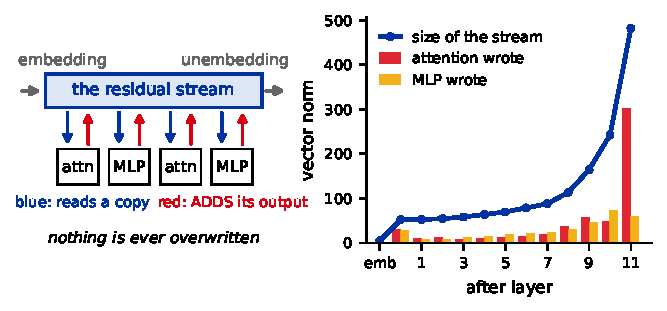
\includegraphics[width=0.99\textwidth]{fig/residual_stream.pdf}
  \end{center}
  \vspace{-0.5em}
  {\footnotesize Right: GPT-2 small, last position, averaged over our 64 sentences. Each layer
  writes twice; the embedding plus all 24 writes rebuilds the final vector with \textbf{zero
  error}.}
\end{frame}

\begin{frame}{Everything is a sum}
  \vspace{0.8em}
  Nothing overwrites the stream. Each component \textbf{adds}. Split each attention layer into its
  12 heads, and the vector that arrives at the output is nothing more than:

  \vspace{0.8em}
  \[
    \underbrace{\text{final residual}}_{\text{768 numbers}} \;=\;
    \underbrace{e_{\text{tok}} + e_{\text{pos}}}_{\text{the embeddings}} \;+\;
    \underbrace{\sum_{\text{144 heads}} h_i}_{\text{what each head wrote}} \;+\;
    \underbrace{\sum_{\text{12 MLPs}} m_j}_{\text{what each MLP wrote}} \;+\;
    \underbrace{b}_{\text{a constant}}
  \]

  \vspace{0.6em}
  One long sum with \textbf{159 terms}: the token and the position embedding, 144 heads, 12 MLPs,
  and $b$ - the attention layers' output biases, added the same way whatever the input. That is
  the entire architecture, from the point of view of this chapter.

  \vspace{0.5em}
  And the terms are not small. Averaged over our 64 sentences, the stream leaves the embedding
  with norm \textbf{4.5} and reaches the unembedding at \textbf{482}: the layers write about a
  hundred times more into it than the tokens did.
\end{frame}

\begin{frame}{The metric: logit difference}
  \vspace{0.7em}
  Our sentence has exactly two plausible answers and only one is right. So compare them
  directly:

  \vspace{0.7em}
  \[
    \text{logit difference} \;=\;
      \underbrace{\text{logit}(\text{`` William''})}_{\text{correct}} \;-\;
      \underbrace{\text{logit}(\text{`` Alex''})}_{\text{the other name}}
  \]

  \vspace{1.0em}
  \begin{columns}[T]
    \begin{column}{0.48\textwidth}
      \textbf{Why not accuracy?}\\[0.3em]
      \small A step function. It cannot tell you a change made the model \emph{slightly} less
      sure - and most changes do exactly that.
    \end{column}
    \begin{column}{0.48\textwidth}
      \textbf{Why not loss?}\\[0.3em]
      \small Loss mixes in all 50{,}257 tokens. We want the one comparison the task is about,
      and nothing else.
    \end{column}
  \end{columns}
\end{frame}

\begin{frame}{A stream two numbers wide}
  \vspace{0.2em}
  Before GPT-2's 768 numbers, a stream with \textbf{two}. Three components write into it, and
  two candidate tokens read out of it:

  \vspace{0.5em}
  \begin{columns}[T]
    \begin{column}{0.46\textwidth}
      \small
      \begin{tabular}{@{}lr@{}}
        \toprule
        embedding writes & $(1,\; 0)$\\
        a head writes & $(0.5,\; 1)$\\
        an MLP writes & $(1.5,\; -0.5)$\\
        \midrule
        \textbf{final stream} & $\mathbf{(3,\; 0.5)}$\\
        \bottomrule
      \end{tabular}

      \vspace{0.6em}
      Unembedding: token A reads the first number, token B the second.
    \end{column}
    \begin{column}{0.5\textwidth}
      \small
      logit(A) $= 3$, \quad logit(B) $= 0.5$\\[0.3em]
      logit difference $= 3 - 0.5 = \mathbf{2.5}$

      \vspace{0.6em}
      Now split it by who wrote what:\\[0.3em]
      embedding: $1 - 0 = 1$\\
      head: $0.5 - 1 = -0.5$\\
      MLP: $1.5 - (-0.5) = 2$\\[0.3em]
      total: $1 - 0.5 + 2 = \mathbf{2.5}$ \textcolor{paramgreen}{\ding{51}}
    \end{column}
  \end{columns}

  \vspace{0.7em}
  \keybox{\small Because the stream is a sum and reading it out is linear, every component gets its
  own share of the answer. Here the MLP did the work and the head pushed \emph{against} it. The
  same bookkeeping, with 159 terms, is what the next four slides do to GPT-2.}
\end{frame}

\begin{frame}{One sentence, by hand}
  \vspace{0.5em}
  \promptbox{``Then, Alex and William went to the restaurant. Alex gave a book to \ldots''}

  \vspace{0.2em}
  The model's top five predictions for the next token, with their logits:

  \vspace{0.4em}
  \begin{center}
  \small
  \begin{tabular}{@{}lr@{}}
    \toprule
    \textbf{token} & \textbf{logit}\\
    \midrule
    \textcolor{paramgreen}{\textbf{`` William''}} & \textcolor{paramgreen}{\textbf{17.96}}\\
    `` the'' & 15.50\\
    `` his'' & 14.79\\
    `` them'' & 13.96\\
    `` a'' & 13.69\\
    \midrule
    \textcolor{armred}{`` Alex''} & \textcolor{armred}{12.62}\\
    \bottomrule
  \end{tabular}
  \end{center}

  \vspace{0.1em}
  \[
    \text{logit difference} \;=\; 17.96 \;-\; 12.62 \;=\; \mathbf{5.34}
  \]

  \vspace{-0.3em}
  {\footnotesize Across 64 such sentences the average is \textbf{+3.60}; we always quote the
  average.}
\end{frame}

\begin{frame}{So the logit difference is a sum too}
  \vspace{0.8em}
  The step from the residual stream to a logit is a \textbf{matrix multiply} - the unembedding.
  Matrix multiplication is linear, and linear means it distributes over a sum:

  \vspace{0.2em}
  \[
    W_U \big( a + b + c \big) \;=\; W_U a \;+\; W_U b \;+\; W_U c
  \]

  \vspace{0.2em}
  Apply that to the 159-term sum from before, and the logit difference splits the same way:

  \vspace{0.2em}
  \[
    \text{logit difference} \;=\;
      \underbrace{c_{\text{tok}} + c_{\text{pos}} + c_{\text{L0H0}} + \cdots + c_{\text{L11H11}}
      + \cdots}_{\text{one number per component}}
  \]

  \vspace{0.5em}
  \keybox{Each component gets a \textbf{single number}: how much it pushed toward `` William''
  over `` Alex''. That number is the component's \textbf{direct logit attribution}.}
\end{frame}

\begin{frame}{Do not take my word for it}
  \vspace{0.1em}
  \begin{center}
    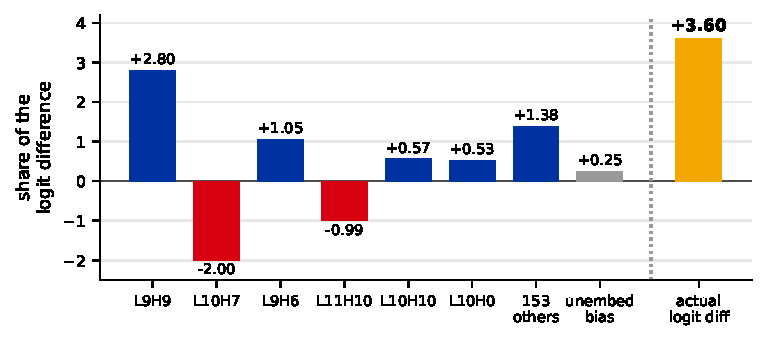
\includegraphics[width=0.9\textwidth]{fig/logit_decomposition.pdf}
  \end{center}
  \vspace{-0.4em}
  {\footnotesize Averaged over our 64 sentences: the six largest of the 159 terms, the other 153
  lumped together, then GPT-2's unembedding bias - a fixed offset the model does not compute.
  Orange is the logit difference from an ordinary forward pass. Red bars push \emph{against}
  the right answer.}
\end{frame}

\begin{frame}{The sum is exact}
  \vspace{0.8em}
  \begin{center}
  \small
  \begin{tabular}{@{}lr@{}}
    \toprule
    159 component contributions, added up & $+3.3439$\\
    unembedding bias (a constant, not computed by the model) & $+0.2520$\\
    \midrule
    \textbf{total} & $\mathbf{+3.5960}$\\
    logit difference from an ordinary forward pass & $+3.5960$\\
    \midrule
    \textbf{difference} & $\mathbf{0.00000}$\\
    \bottomrule
  \end{tabular}
  \end{center}

  \vspace{0.5em}
  \takebox{\textbf{This is why per-component attribution exists at all.} ``How much did L9H9
  contribute?'' has an exact answer, because the architecture really is a sum. Remove the
  residual connections and most of this chapter stops working.}

  \vspace{0.6em}
  {\footnotesize One honest caveat: LayerNorm sits between the stream and the unembedding and
  is \emph{not} linear. We hold its scaling factor fixed at the value the real forward pass
  produced - which is what makes the table above come out exact.}
\end{frame}

\begin{frame}{The one piece of code in this lecture}
  \vspace{0.6em}
  \codebox{%
    logits, cache = model.run\_with\_cache("Then, Alex and William went to the\ldots")\\[0.4em]
    cache["resid\_post", 9]\hspace{2.6em}\# the stream after layer 9\\
    cache["pattern", 9]\hspace{3.9em}\# attention weights, all 12 heads\\
    cache["z", 9]\hspace{5.5em}\# what each head wrote
  }

  \vspace{0.5em}
  One forward pass, and every intermediate value is kept instead of thrown away. That is the
  whole trick, and it is why libraries like TransformerLens exist: not new mathematics, just
  refusing to discard the activations.

  \vspace{0.8em}
  \watchbox{Most of the practical difficulty in this field is \textbf{careful indexing} - which
  layer, which position, which head. Not the concepts. Budget your frustration accordingly.}
\end{frame}

% ============================================================ SECTION 2
\section{The logit lens}
\sectiontransition{The logit lens}{If the answer is built gradually, can we watch it happen?}

\begin{frame}{One idea, one sentence}
  \vspace{0.9em}
  \keybox{Take the residual stream \textbf{halfway through} the model, apply the unembedding
  that is normally used only at the end, and read off what the model \textbf{would have said}
  if it had stopped there.}

  \vspace{0.9em}
  Nothing about this is principled - we are applying the final layer's decoder to a vector it
  was never trained to decode. It works well enough on GPT-2 to be useful, which is a sentence
  that should already make you slightly suspicious. We will return to that.

  \vspace{0.7em}
  {\footnotesize Introduced by nostalgebraist (2020), as a blog post rather than a paper - which
  is common in this field.}
\end{frame}

\begin{frame}{Predict first}
  \vspace{1.0em}
  We are about to run the logit lens at every layer of GPT-2 small and plot the logit difference
  as it develops.

  \vspace{1.4em}
  \begin{center}
    {\large Sketch the shape of that curve before you see it.}\\[0.7em]
    {\normalsize Does the answer build up \textbf{steadily} across the twelve layers,\\
     or does it arrive \textbf{somewhere in particular}?}
  \end{center}

  \vspace{1.4em}
  \begin{center}
    {\footnotesize Most people draw a diagonal line. Very few draw what actually happens.}
  \end{center}
\end{frame}

\begin{frame}{Watching the answer arrive}
  \vspace{0.1em}
  \begin{center}
    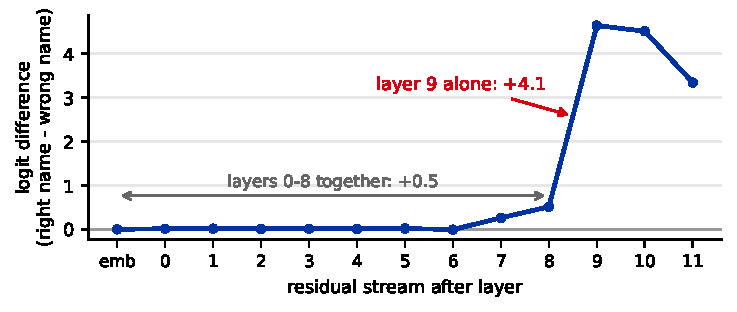
\includegraphics[width=0.87\textwidth]{fig/logit_lens.pdf}
  \end{center}
  \vspace{-0.5em}
  \begin{columns}[T]
    \begin{column}{0.55\textwidth}
      {\footnotesize
      \begin{itemize}\itemsep2pt
        \item Layers 0-8, \textbf{all nine together}: $+0.5$.
        \item \textbf{Layer 9 alone}: $+4.1$.
        \item Layers 10 and 11 take some back: $+3.3$ at the end.
      \end{itemize}}
    \end{column}
    \begin{column}{0.43\textwidth}
      {\footnotesize Read off the stream after each layer, averaged over 64 sentences; ``emb'' is
      before any layer. It ends at $+3.3$, not $+3.6$: the lens leaves out the unembedding bias.}
    \end{column}
  \end{columns}
\end{frame}

\begin{frame}{Not just this sentence}
  \vspace{-0.3em}
  \begin{center}
    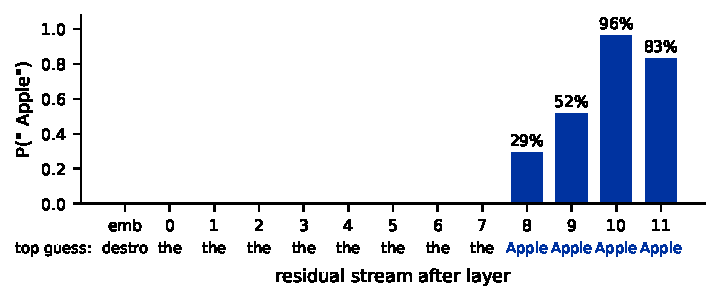
\includegraphics[width=0.85\textwidth]{fig/l45_lens_fact.pdf}
  \end{center}
  \vspace{-0.7em}
  {\small A completely different task: ``Steve Jobs was the founder of''. After layer 7 the
  model's best guess is still `` the'', and `` Apple'' is ranked \textbf{22nd}. Layer 8 puts it
  first.}

  \vspace{0.3em}
  {\footnotesize Two sentences are not a law of nature - but it is the same shape, one layer
  earlier: the early layers do not say the answer, one late layer does. (And the very last layer
  \emph{lowers} the confidence, from 96\% to 83\%.)}
\end{frame}

\begin{frame}{One number to carry forward}
  \vspace{1.0em}
  \keybox{The decision is \textbf{not} spread evenly through the network. Something specific
  happens at \textbf{layer 9}, and whatever it is, it is responsible for most of the answer.}

  \vspace{1.0em}
  That is our first real hypothesis, and it is narrow enough to test: \textbf{look at layer 9}.

  \vspace{1.2em}
  \takebox{Remember the number. In the causal-methods lecture we go looking for the components that
  do this work, using a completely different method that knows nothing about this graph.\\[0.4em]
  They will be in \textbf{layer 9}.}
\end{frame}

\begin{frame}{Before you trust it}
  \vspace{0.6em}
  \trapbox{The logit lens is \textbf{not} a window into ``what the model is thinking''. It is a
  decoder being used out of distribution.}

  \vspace{0.8em}
  \begin{itemize}
    \item It works reasonably on GPT-2 and \textbf{poorly on many other models} - representations
      drift between layers, and the final unembedding does not match them.
    \item The fix people use - training a small decoder per layer, the ``tuned lens'' (Belrose et
      al., 2023) - exists precisely because the plain version is unreliable.
    \item It shows what is \textbf{linearly readable}, which is not the same as what is
      \textbf{there}, which is not the same as what is \textbf{used}.
  \end{itemize}

  \vspace{0.7em}
  That last distinction is important enough that the next section is about nothing else.
\end{frame}

% ============================================================ SECTION 3
\section{Probes}
\sectiontransition{Probes}{Asking the model a yes/no question about its own activations}

\begin{frame}{A probe is logistic regression}
  \vspace{0.6em}
  You already know how to build one. From lecture 11:

  \vspace{0.5em}
  \begin{center}
  \small
  \begin{tabular}{@{}ll@{}}
    \toprule
    \textbf{Lecture 11} & \textbf{Here}\\
    \midrule
    design matrix of features & the residual stream, 768 numbers per token\\
    label: is this cheese batch bad? & label: is one of these names repeated?\\
    fit logistic regression & fit logistic regression\\
    \bottomrule
  \end{tabular}
  \end{center}

  \vspace{0.8em}
  \keybox{Train a classifier on activations. If it succeeds, that information is present in the
  stream in a \textbf{linearly readable} form. That is the whole method.}

  \vspace{0.6em}
  We train one probe per layer, cross-validated, on 128 sentences balanced 50/50 between
  ``a name repeats'' and ``three different names''.
\end{frame}

\begin{frame}{What ``linearly readable'' looks like}
  \vspace{-0.3em}
  \begin{center}
    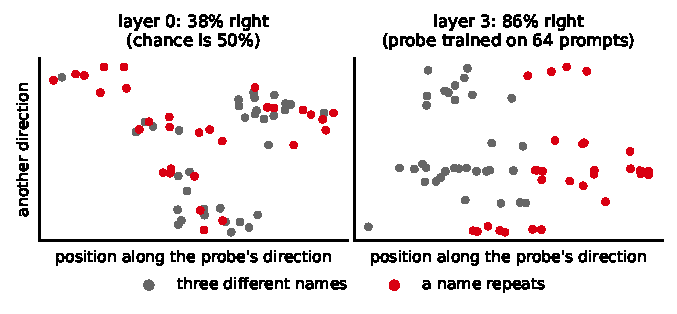
\includegraphics[width=0.8\textwidth]{fig/l45_probe_picture.pdf}
  \end{center}
  \vspace{-0.6em}
  {\small Each dot is a prompt the probe has \textbf{never seen}, placed by the stream at its last
  position. Train a probe on half the prompts, then project the other half onto its direction.}

  \vspace{0.3em}
  {\small At layer 0 the two kinds of prompt are mixed together. At layer 3 a single straight cut
  along one direction puts most of them on the right side. That is all ``linearly readable''
  means.}
\end{frame}

\begin{frame}{Predict first}
  \vspace{1.0em}
  We train one probe per layer, asking only: \emph{is one of these names repeated?}

  \vspace{1.3em}
  \begin{center}
    {\large At which layer do you think the probe first hits 100\%?}
  \end{center}

  \vspace{1.3em}
  \begin{columns}[T]
    \begin{column}{0.5\textwidth}
      \centering Late, near layer 9, where we just saw the answer appear?
    \end{column}
    \begin{column}{0.5\textwidth}
      \centering Or somewhere else entirely?
    \end{column}
  \end{columns}

  \vspace{1.2em}
  \begin{center}
    {\footnotesize Commit to a layer number before the next slide.}
  \end{center}
\end{frame}

\begin{frame}{The information shows up early}
  \vspace{0.2em}
  \begin{center}
    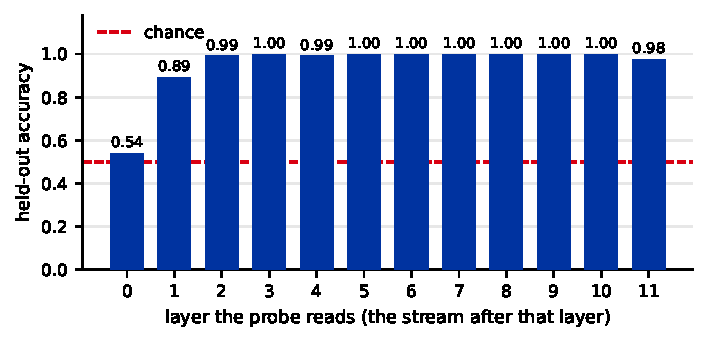
\includegraphics[width=0.84\textwidth]{fig/probe_by_layer.pdf}
  \end{center}
  \vspace{-0.4em}
  {\footnotesize Five-fold cross-validated accuracy (always on prompts the probe did not train on),
  one probe per layer, reading the last position. \textbf{100\% first at layer 3}, and 98-100\% at
  every layer after - six layers before the model does anything with it.}
\end{frame}

\begin{frame}{The two graphs, together}
  \vspace{0.1em}
  \begin{center}
    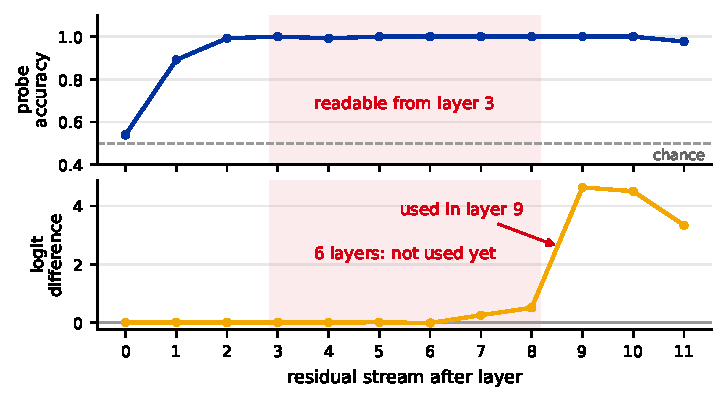
\includegraphics[width=0.86\textwidth]{fig/probe_vs_lens.pdf}
  \end{center}
  \vspace{-0.5em}
  {\footnotesize Same $x$ axis: the stream after each layer. Top: what is \textbf{readable}.
  Bottom: what is \textbf{used}.}
\end{frame}

\begin{frame}{Six layers of knowing and not acting}
  \vspace{1.0em}
  \trapbox{\textbf{The information sat in the residual stream, 98-100\% readable, from layer 3
  on - and the model's answer did not move until layer 9.}}

  \vspace{1.0em}
  \keybox{A probe tells you a fact is \textbf{present}. It does not tell you the model
  \textbf{uses} it.}

  \vspace{1.0em}
  You can read every ingredient off a label without knowing which ones the recipe calls for. The
  probe reads the label. It has nothing to say about the cooking.

  \vspace{0.9em}
  {\footnotesize This gap is the single most useful thing in the lecture, because it is the
  mistake people actually make: finding information with a probe and reporting it as what the
  model is \emph{doing}.}
\end{frame}

\begin{frame}{How a probe can fool you}
  \vspace{0.5em}
  \begin{itemize}
    \item \textbf{Presence is not use} - the six-layer gap above, measured on our own data.
    \item \textbf{The probe may be doing the work.} Measured: give the layer-3 probe
      \emph{shuffled} labels - pure noise - and it still gets \textbf{80\%} of its own training
      prompts right. On new prompts: \textbf{44\%}. With 768 numbers per prompt and only 128
      prompts, a probe can memorise noise. Keep probes linear, and only ever report accuracy on
      prompts it did not train on.
    \item \textbf{Correlated features.} The probe may be reading something that merely travels
      with what you asked about.
  \end{itemize}

  \vspace{0.8em}
  \watchbox{Our probe hitting \textbf{100\%} by layer 3 should make you ask whether the task was
  too easy, not congratulate the model. An easy task is fine here, because the point of the
  figure is the \textbf{contrast} with the logit lens - not the accuracy.}
\end{frame}

\begin{frame}{Where probes actually earn their keep}
  \vspace{0.6em}
  \textbf{Othello-GPT.} Train a transformer only on sequences of legal Othello moves - it never
  sees a board. Then probe its activations for the state of each square.

  \vspace{0.5em}
  The probes work. The model built an internal \textbf{board} it was never given.

  \vspace{0.9em}
  \keybox{This is the strongest thing probes have shown: models can construct genuine internal
  \textbf{world models} from data that only implies them.}

  \vspace{0.8em}
  And the practical version: linear probes on activations are \textbf{deployed today} for
  content monitoring in real systems. Of everything in this chapter, this is the
  technique most likely to be useful in your job - it is cheap to train, cheap to run, and it
  works.

  \vspace{0.5em}
  {\footnotesize Li et al.\ (2022); the linear-probe follow-up is Nanda et al.\ (2023).}
\end{frame}

% ============================================================ SECTION 4
\section{Reading attention heads}
\sectiontransition{Reading attention heads}{144 of them. Which ones are doing the work?}

\begin{frame}{What a head does, restated}
  \vspace{0.7em}
  From the attention lecture in the LLM chapter: a head computes queries, keys and values, and
  produces a weighted sum of values.

  \vspace{0.6em}
  For our purposes, one sentence is enough:

  \vspace{0.6em}
  \keybox{An attention head \textbf{moves information from one position to another}. The
  attention pattern says \emph{where from}; what it writes is a separate question entirely.}

  \vspace{0.9em}
  That split is the whole content of this section. The pattern is easy to look at, easy to
  screenshot, and easy to over-read.
\end{frame}

\begin{frame}{Reading an attention pattern}
  \begin{columns}[T]
    \begin{column}{0.56\textwidth}
      \vspace{-0.6em}
      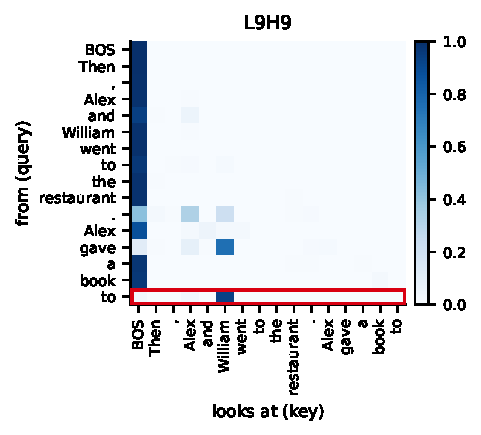
\includegraphics[width=\linewidth]{fig/attention_pattern.pdf}
    \end{column}
    \begin{column}{0.42\textwidth}
      \small
      One head on our sentence. Each \textbf{row} is one position deciding where to look; each
      \textbf{column} is a position it can look at. Every row adds up to 100\%.

      \vspace{0.4em}
      Rows only look \textbf{left}: a token cannot see the future.

      \vspace{0.4em}
      The dark first column: most rows park their attention on BOS (beginning of sequence), the
      token GPT-2 puts first - an \textbf{attention sink}, mostly not about the sentence.

      \vspace{0.3em}
      \keybox{\small The row that matters is the \textbf{last} one (red box): the position that
      predicts the next word.}
    \end{column}
  \end{columns}
\end{frame}

\begin{frame}{Four heads, the row that matters}
  \vspace{-0.2em}
  \begin{center}
    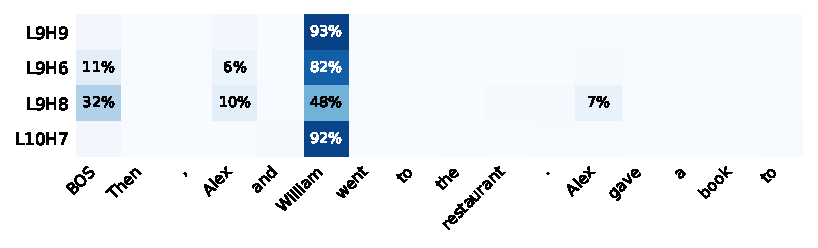
\includegraphics[width=0.96\textwidth]{fig/attention_last_row.pdf}
  \end{center}
  \vspace{-0.6em}
  {\footnotesize Where the last position looks, in four heads: all four, mostly at `` William''.}

  \vspace{0.2em}
  \trapbox{\small Now measure what two of them \emph{write} on this sentence, with direct logit
  attribution. \textbf{L9H9} (93\% on `` William'') adds $+3.81$ to the logit difference.
  \textbf{L10H7} (92\% on `` William'') adds $-2.59$: it pushes \textbf{against} the right answer.
  Same picture, opposite effect.}
\end{frame}

\begin{frame}{Where it looks is not what it writes}
  \vspace{0.5em}
  A head does two separable things, and we can only see one of them:

  \vspace{0.7em}
  \begin{center}
  \small
  \begin{tabular}{@{}>{\raggedright\arraybackslash}p{0.24\textwidth}>{\raggedright\arraybackslash}p{0.32\textwidth}>{\raggedright\arraybackslash}p{0.36\textwidth}@{}}
    \toprule
    & \textbf{Where it looks} & \textbf{What it writes}\\
    \midrule
    Set by & queries and keys & values, and the output matrix\\[0.3em]
    Shown by & the attention pattern & \textcolor{armred}{nothing you can look at}\\[0.3em]
    Easy to plot? & yes - it is a heatmap & no - it is a 768-dimensional vector\\
    \bottomrule
  \end{tabular}
  \end{center}

  \vspace{0.6em}
  \trapbox{\small Every attention picture you have ever seen - including the four on the last
  slide - shows only the \textbf{left} column. A head can stare straight at the right answer and
  write a vector that no later component reads.}

  \vspace{0.4em}
  {\small Direct attribution shows what a head writes straight into the answer. Whether a later
  part \emph{reads} it is a causal question - that is the causal-methods lecture.}
\end{frame}

\begin{frame}{Induction heads}
  \vspace{0.5em}
  The most famous named circuit in the field, and it is easy to state:

  \vspace{0.6em}
  \promptbox{\ldots\ \textbf{A} \textbf{B} \ldots\ \textbf{A} $\rightarrow$ predict \textbf{B}}

  \vspace{0.3em}
  \emph{``This pattern appeared before. What came next last time?''}

  \vspace{0.7em}
  Test it with a sequence of \textbf{random} tokens repeated twice. There is nothing to learn
  from the language - the only way to predict the second half is to look back at the first.

  \vspace{0.7em}
  \keybox{It is why a model can pick up a pattern you invent inside a single prompt. Olsson et
  al.\ go further and argue it may be most of how large models learn in context - on evidence
  they themselves call preliminary.}

  \vspace{0.4em}
  {\footnotesize Olsson et al.\ (2022), \emph{In-context Learning and Induction Heads}.}
\end{frame}

\begin{frame}{Walk through it, one position at a time}
  \vspace{0.4em}
  A concrete sequence. The model has seen the first four tokens and must predict the fifth:

  \vspace{0.6em}
  \begin{center}
  \begin{tikzpicture}[font=\small]
    \foreach \i/\t in {0/\texttt{cat}, 1/\texttt{sat}, 2/\texttt{dog}, 3/\texttt{cat}} {
      \node[draw, rounded corners=2pt, minimum width=1.5cm, minimum height=0.75cm,
            fill=lightbg] (t\i) at (\i*1.85, 0) {\t};
      \node[font=\scriptsize, gray] at (\i*1.85, -0.62) {position \i};
    }
    \node[draw, rounded corners=2pt, minimum width=1.5cm, minimum height=0.75cm,
          fill=armorange!15, dashed] (q) at (4*1.85, 0) {\texttt{?}};
    \node[font=\scriptsize, gray] at (4*1.85, -0.62) {position 4};
  \end{tikzpicture}
  \end{center}

  \vspace{0.9em}
  The answer a human gives instantly: \textbf{\texttt{sat}}. The pattern \texttt{cat} appeared
  before, and \texttt{sat} followed it.

  \vspace{0.9em}
  The model has no rule for this. What it has is two heads, in two different layers, and neither
  of them can do it alone.
\end{frame}

\begin{frame}{Step 1 - the previous-token head}
  \vspace{0.6em}
  In an \textbf{early} layer, one head does something that looks pointless: at every position, it
  attends to the position \emph{before} it, and copies that token's identity into the stream.

  \vspace{0.7em}
  \begin{center}
  \begin{tikzpicture}[font=\small]
    \foreach \i/\t in {0/\texttt{cat}, 1/\texttt{sat}, 2/\texttt{dog}, 3/\texttt{cat}} {
      \node[draw, rounded corners=2pt, minimum width=1.45cm, minimum height=0.72cm,
            fill=lightbg] (t\i) at (\i*2.2, 0) {\t};
    }
    \draw[-{Latex[length=2mm]}, armblue, thick] (t1.north) to[bend right=32] (t0.north);
    \draw[-{Latex[length=2mm]}, armblue, thick] (t2.north) to[bend right=32] (t1.north);
    \draw[-{Latex[length=2mm]}, armblue, thick] (t3.north) to[bend right=32] (t2.north);
    \node[font=\scriptsize, armblue, align=center] at (1.1, 1.15) {``the token before me\\was
      \texttt{cat}''};
  \end{tikzpicture}
  \end{center}

  \vspace{0.6em}
  So position 1 now carries a \textbf{mark}: \emph{I am preceded by} \texttt{cat}.

  \vspace{0.5em}
  {\footnotesize On its own this is useless. It is bookkeeping done in advance, by a head that
  has no idea what it will be used for.}
\end{frame}

\begin{frame}{Step 2 - the induction head}
  \vspace{0.5em}
  In a \textbf{later} layer, a second head sits at the final position, whose token is
  \texttt{cat}, and asks the stream a question:

  \vspace{0.2em}
  \begin{center}
    \emph{``Which earlier position is marked as being preceded by \texttt{cat}?''}
  \end{center}

  \vspace{0.2em}
  \begin{center}
  \begin{tikzpicture}[font=\small]
    \foreach \i/\t in {0/\texttt{cat}, 1/\texttt{sat}, 2/\texttt{dog}, 3/\texttt{cat}} {
      \node[draw, rounded corners=2pt, minimum width=1.45cm, minimum height=0.72cm,
            fill=lightbg] (t\i) at (\i*2.2, 0) {\t};
    }
    \node[draw, rounded corners=2pt, minimum width=1.45cm, minimum height=0.72cm,
          fill=armorange!15, dashed] (q) at (4*2.2, 0) {\texttt{?}};
    \draw[-{Latex[length=2mm]}, paramgreen, very thick] (q.south) to[bend left=25] (t1.south);
    \node[font=\scriptsize, paramgreen] at (4.4, -1.45) {position 1 is the match - copy its
      token};
  \end{tikzpicture}
  \end{center}

  \vspace{0.4em}
  Position 1 is marked. Its token is \texttt{sat}. The head copies \texttt{sat} to the output.

  \vspace{0.3em}
  \keybox{The mark was written by a head that did not know why. It was read by a head that never
  saw the original \texttt{cat}. \textbf{Neither one contains the algorithm.}}
\end{frame}

\begin{frame}{That is what ``circuit'' means}
  \vspace{0.7em}
  \begin{center}
  \begin{tikzpicture}[font=\small]
    \node[draw, rounded corners, fill=armblue!10, minimum width=4.0cm, minimum height=1.25cm,
          align=center] (prev) at (0,0) {\textbf{previous-token head}\\[0.2em]
          \scriptsize early layer\\[-0.05em]\scriptsize writes the mark};
    \node[draw, rounded corners, fill=paramgreen!10, minimum width=4.0cm, minimum height=1.25cm,
          align=center] (ind) at (7.4,0) {\textbf{induction head}\\[0.2em]
          \scriptsize later layer\\[-0.05em]\scriptsize reads it, copies what followed};
    \draw[-{Latex[length=2.5mm]}, thick] (prev) -- (ind);
    \node[font=\scriptsize, align=center] at (3.7, 0.42) {via the};
    \node[font=\scriptsize, align=center] at (3.7, -0.42) {residual stream};
  \end{tikzpicture}
  \end{center}

  \vspace{1.0em}
  \takebox{A \textbf{circuit} is a behaviour that lives in the \emph{composition} of components,
  not in any one of them. Delete either head and the behaviour disappears - but you will never
  find it by examining either head alone.}

  \vspace{0.8em}
  This is why ``which neuron represents X'' is so often the wrong question, and it is the shape
  of every result in the causal-methods lecture.
\end{frame}

\begin{frame}{Finding them, in one pass}
  \vspace{0.1em}
  \begin{center}
    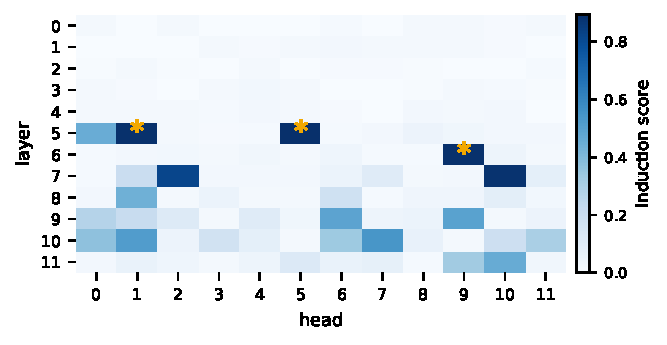
\includegraphics[width=0.78\textwidth]{fig/induction_scores.pdf}
  \end{center}
  \vspace{-0.4em}
  {\footnotesize Induction score: 40 random tokens, repeated. How much attention each token in the
  second copy puts on the token that came \emph{after} it the first time (1 = all of it). Top three
  (stars): \textbf{L5H5}, \textbf{L6H9}, \textbf{L5H1}, all 0.89 - the middle of the model.}
\end{frame}

\begin{frame}{Predict first}
  \vspace{0.9em}
  We have found a head whose attention pattern is exactly what an induction head should look
  like.

  \vspace{1.1em}
  \begin{center}
    {\large Does that prove the head is \textbf{doing} induction?}
  \end{center}

  \vspace{1.1em}
  \pause
  No.

  \vspace{0.5em}
  \trapbox{A head can attend somewhere and write \textbf{nothing useful} when it gets there.
  Attention says where a head \emph{looked}. It says nothing about what it \emph{did}, or
  whether anything downstream \textbf{read} the result.}

  \vspace{0.6em}
  The causal-methods lecture opens with three heads in one layer, all looking at the right answer.
  One contributes nothing, and the pictures will not tell you which.
\end{frame}

% ============================================================ SECTION 5
\section{Naming what you find}
\sectiontransition{Naming what you find}{The most natural thing to do, and the easiest way to be wrong}

\begin{frame}{Max-activating examples}
  \vspace{0.6em}
  The standard way to name a neuron or a head: run a lot of text through, keep the inputs that
  make it fire hardest, and look at them.

  \vspace{0.7em}
  \begin{center}
  \begin{tcolorbox}[colback=lightbg, colframe=gray, boxrule=0.5pt, arc=2pt, width=0.9\textwidth]
    \small
    Top activations for a neuron {\footnotesize\color{gray}(an illustration, not a measured
    neuron)}:\\[0.3em]
    \footnotesize
    \ldots{} the \textbf{Golden Gate} Bridge \ldots\\
    \ldots{} crossing the \textbf{bridge} at dawn \ldots\\
    \ldots{} San Francisco's famous \textbf{span} \ldots
  \end{tcolorbox}
  \end{center}

  \vspace{0.5em}
  It is genuinely useful, it is how most features get named, and it has a failure mode serious
  enough to have its own name. First, why it happens.
\end{frame}

\begin{frame}{Most neurons are not about one thing}
  \vspace{0.6em}
  Look at enough GPT-2 neurons and the pattern is unmistakable: a single neuron fires on
  several \textbf{unrelated} concepts.

  \vspace{0.8em}
  \keybox{\textbf{Polysemanticity.} One neuron, many meanings. It is the normal case, not the
  exception - which means ``find the neuron for X'' is usually the wrong question.}

  \vspace{0.9em}
  You have met the reason already: in the autoencoder chapter, a network had to track 40 word
  identities in 32 dimensions, and had no choice but to share directions. We return to it
  properly in the features lecture, where it stops being a nuisance and becomes the organising
  idea.
\end{frame}

\begin{frame}{The interpretability illusion}
  \vspace{0.6em}
  Bolukbasi et al.\ (2021) took a neuron in BERT, collected its top-activating examples on one
  dataset, and got a clean, convincing story.

  \vspace{0.5em}
  Then they ran a \textbf{different} dataset through the same neuron and got a different clean,
  convincing story.

  \vspace{0.9em}
  \trapbox{Both stories were supported by the evidence. At most one of them was right.
  \textbf{Cherry-picking is not a mistake you might make here - it is the default behaviour of
  the method.}}

  \vspace{0.8em}
  The defence is dull and non-negotiable: report \textbf{randomly selected} examples alongside
  the top ones, and check across datasets.
\end{frame}

% ============================================================ RECAP
\begin{frame}{Recap}
  \vspace{0.4em}
  \begin{center}
  \small
  \begin{tabular}{@{}>{\raggedright\arraybackslash}p{0.24\textwidth}>{\raggedright\arraybackslash}p{0.39\textwidth}>{\raggedright\arraybackslash}p{0.31\textwidth}@{}}
    \toprule
    \textbf{Technique} & \textbf{What it told us} & \textbf{What it cannot tell us}\\
    \midrule
    Residual stream & everything is a sum, so attribution is possible & -\\[0.3em]
    Logit lens & the answer appears in layer 9 & whether layer 9 \emph{causes} it\\[0.3em]
    Probes & duplication is readable from layer 3 & whether the model uses it\\[0.3em]
    Attention patterns & heads look at the right names & whether looking mattered\\[0.3em]
    Max-activating examples & a name for a component & whether the name is correct\\
    \bottomrule
  \end{tabular}
  \end{center}

  \vspace{0.7em}
  \trapbox{Read the right-hand column again. \textbf{Every technique in this lecture is
  correlational.} We have four ways to form a hypothesis and not one way to test one.}
\end{frame}

\begin{frame}{Next}
  \vspace{1.2em}
  \takebox{\textbf{Next: intervention.}\\[0.6em]
  Instead of watching the model run, we \textbf{break} it on purpose - delete a head, swap an
  activation, and measure what changes. That is the difference between noticing that something
  looks important and showing that it \textbf{is}.\\[0.8em]
  We open with three heads that all look right. One of them does nothing.}

  \vspace{1.0em}
  \begin{center}
    {\footnotesize Optional, after the core lectures: \emph{Circuits read off the weights} - the
    induction circuit from this lecture, found in the weights alone without running any
    text.\\[0.3em]
    Optional viewing: the Welch Labs video on grokking, linked on the chapter page - a complete
    circuit, in a model small enough to understand entirely.}
  \end{center}
\end{frame}

\end{document}

% Provenance:
% - Source material: Neel Nanda, "How To Become A Mechanistic Interpretability Researcher"
%   (minimum-viable-basics list: patching, probes, SAEs, max-activating examples); ARENA
%   chapter 1.2; Elhage et al. (2021) "A Mathematical Framework for Transformer Circuits"
%   (residual stream as shared channel); nostalgebraist (2020) logit lens; Olsson et al. (2022)
%   induction heads; Li et al. (2022) + Nanda et al. (2023) Othello-GPT; Bolukbasi et al.
%   interpretability illusion for BERT.
% - Figures: logit_lens, probe_by_layer, attention_pattern, attention_last_row, induction_scores
%   from py_src/l45_figs.py (GPT-2 small, CPU, data/ioi_dataset.json -> results/l45_figs.json);
%   logit_decomposition + probe_vs_lens from l45_extra_figs.py; residual_stream from
%   l45_residual_stream.py; l45_lens_fact + l45_probe_picture from l45_easy_figs.py. All four
%   scripts take --plot-only and redraw from results/*.json. Every GPT-2 number on a slide is
%   measured; the two-wide toy stream and the max-activating box are illustrations, labelled.
% - Key pedagogical decisions:
%   (1) The deck deliberately ENDS IN FAILURE - every technique shown is correlational, and the
%       recap says so. That cliffhanger is the motivation for L46 and must not be softened.
%   (2) The probe/logit-lens contrast (readable at layer 3, used at layer 9) replaces the
%       planned "ingredients on a label" analogy. It is the same lesson, measured instead of
%       asserted, and it emerged from the data rather than being designed in.
%   (3) The cold open argues AGAINST the chapter twice - the black-box comparison table, and the
%       "why a small old model" frame that pre-empts the toy-model tension L46 raises. Added
%       after review; the first draft argued only for the field.
%   (4) Layer 9 is planted here by the logit lens and paid off in L46 by direct logit
%       attribution - two independent methods, same answer, neither told about the other.
% - Revised 2026-09-22 (ch19 extension, EXTENSION_PLAN.md task 2, "moderate"): the five
%   chapter-level cold-open frames moved to 01_mech_interp_intro.tex; the cold open is now a recap,
%   the IOI sentence (probability 74% measured in intro_figs.py), a model spec table and a
%   glossary. Added: a width-2 toy stream decomposed by hand; the logit lens on a second task
%   (fig/l45_lens_fact.pdf: " Apple" rank 22 after layer 8, first after layer 9); the held-out
%   probe picture (fig/l45_probe_picture.pdf) and the shuffled-label control (80% in-sample, 44%
%   5-fold CV) - all from py_src/l45_easy_figs.py -> results/l45_easy_figs.json. "Next lecture"
%   references became lecture titles because optional decks may sit in between.
% - Revised 2026-10-17 (renamed xx_ -> 02_, DECISIONS.md #90; polish pass #91):
%   * Layer indexing made consistent: every layer axis is "emb, 0..11" = the stream after layer L,
%     layers counted from 0 like the head names (mi_common.stream_ticks). The logit-lens figure
%     printed TransformerLens's "9_pre" labels, and the Apple frame said "22nd after layer 8, first
%     after layer 9" while its data (results/l45_easy_figs.json: rank 22 at 8_pre, first at 9_pre)
%     means after layer 7 / layer 8 - one layer earlier than IOI's jump, not the same layer.
%   * "157 terms" (embedding as one term, biases left out) vs "159" on the exact-sum table: the
%     sum frame now lists all 159 (tok + pos embedding, 144 heads, 12 MLPs, attention output
%     biases), matching TransformerLens's get_full_resid_decomposition.
%   * Stale lecture numbers ("lecture 24" = old L24_attention, "lecture 25") replaced by titles;
%     lecture 11's example is the cheese factory, not "did the customer subscribe?".
%   * The four-head attention strip (2.7 pt labels) became two frames: one full pattern (how to
%     read one) and the last row of four heads, with L10H7's measured DLA on this sentence
%     (-2.59 vs L9H9 +3.81) as "same picture, opposite effect". L9H8's DLA (+0.10) is in the JSON
%     but deliberately NOT on a slide: it answers deck 3's cold-open puzzle.
%   * Every figure redrawn at slot size (was 8 pages under 5.5 pt, down to 2.7 pt); 9 overfull
%     frames and the Step 2 box sitting on the page number fixed; induction score defined on the
%     slide; Olsson's in-context-learning claim worded as theirs, with their own hedge.
% - Next deck: 03_does_it_actually_do_that.tex (ablation, patching, DLA, the IOI circuit,
%   self-repair). Its cold open is the three-head figure promised on the last two frames here.
